\subsection{Data Querying} \label{sec:data-query}


\todo[inline]{authentication needed}
\subsubsection{Scenario}
It has been two weeks since Alice from Subsection~\ref{sec:data-insert} published the processed (i.e. indexed) axolotl genome. In fact, she completely forgot that she did insert this data into the Hydra instance on FABRIC. When Alice received an error for trying to insert new data with the same name, she remembered about her forgotten inserted file. From Alice's perspective, having some way of querying to see what files are in Hydra and what file metadata is under a certain name is extremely useful. To satisfy this scenario, the following interactions are conducted.


\subsubsection{User-to-Node Interaction}
The process of how a user sends a query to a Hydra node can be described as a single Interest and a corresponding data packet. Any Hydra node can handle a query sent by the user. The naming of a query interest follows the format /<hydra-prefix>/query/<query-type>.


\subsubsection{Module Interaction}
\begin{figure}[!ht]
    \centering
    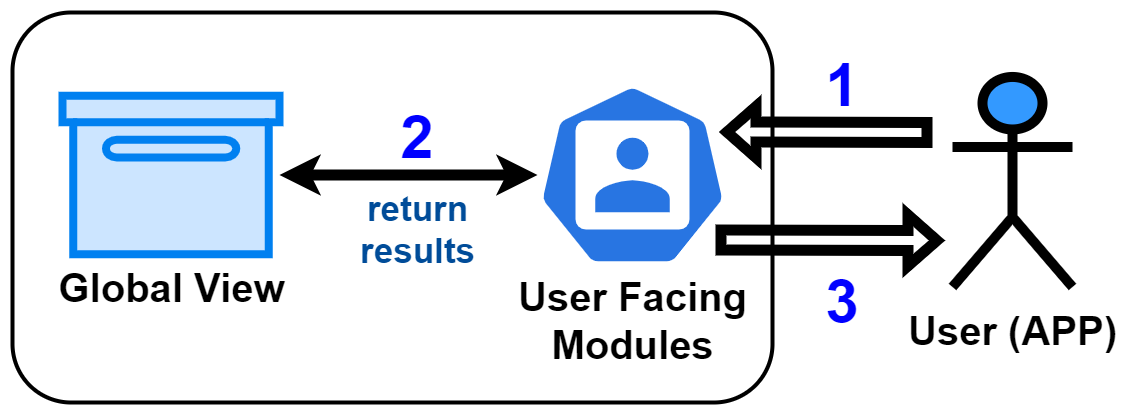
\includegraphics[width=\columnwidth]{visuals/query-sys.png}
    \caption{Module Interaction to Fulfill a User's Query Request}
    \label{fig:query-sys}
\end{figure}

The interest by the user gets processed in a simple way which is described by Figure~\ref{fig:query-sys}. The Hydra node simply checks the Global View for the query type information and returns it via a data packet.


\subsubsection{Types}
There are different query types that are defined. It is important to note that more queries can be added to better suit the environment, but also any queries can be disabled via Hydra's base policy. This gives Hydra instances more flexibility in what they want to expose to the users.

The query types are the following:
\begin{enumerate}
    \item /files: This allows users to see what files are within a Hydra instance. \todo[inline]{authentication?}
    \item /nodes: This allows users to see what nodes are part of a Hydra instance. \todo[inline]{why do users need to know this? I suggest you drop this. This might be a security problem. Yes, only super admins would have this power}
    \item /prefix/<prefix>: This allows users to search Hydra for files under a certain prefix.
    \item /file/<filename>: This allows users to see information about a certain file.
\end{enumerate}